\PassOptionsToPackage{unicode}{hyperref}
\documentclass[aspectratio=1610, 11pt]{beamer}

\usepackage{amsmath}
\usepackage{amssymb}
\usetheme{tudo}

\title{Datenstrukturen, Algorithmen und Programmierung~2}
\author[A.~Coja-Oghlan]{Amin Coja-Oghlan}
\institute[DAP2]{Lehrstuhl Informatik 2\\Fakult\"at f\"ur Informatik}

\newcommand\dist{\mathrm{dist}}
\renewcommand{\vec}[1]{\boldsymbol{#1}}
\newcommand\NULL{{\tt NULL}}
\newcommand\dd{\mathrm d}
\newcommand\eul{\mathrm e}
\newcommand\cA{\mathcal A}
\newcommand\cB{\mathcal B}
\newcommand\cC{\mathcal C}
\newcommand\cD{\mathcal D}
\newcommand\cE{\mathcal E}
\newcommand\cF{\mathcal F}
\newcommand\cG{\mathcal G}
\newcommand\cH{\mathcal H}
\newcommand\cI{\mathcal I}
\newcommand\cJ{\mathcal J}
\newcommand\cK{\mathcal K}
\newcommand\cL{\mathcal L}
\newcommand\cM{\mathcal M}
\newcommand\cN{\mathcal N}
\newcommand\cO{\mathcal O}
\newcommand\cP{\mathcal P}
\newcommand\cQ{\mathcal Q}
\newcommand\cR{\mathcal R}
\newcommand\cS{\mathcal S}
\newcommand\cT{\mathcal T}
\newcommand\cU{\mathcal U}
\newcommand\cV{\mathcal V}
\newcommand\cW{\mathcal W}
\newcommand\cX{\mathcal X}
\newcommand\cY{\mathcal Y}
\newcommand\cZ{\mathcal Z}
\newcommand\fA{\mathfrak A}
\newcommand\fB{\mathfrak B}
\newcommand\fC{\mathfrak C}
\newcommand\fD{\mathfrak D}
\newcommand\fE{\mathfrak E}
\newcommand\fF{\mathfrak F}
\newcommand\fG{\mathfrak G}
\newcommand\fH{\mathfrak H}
\newcommand\fI{\mathfrak I}
\newcommand\fJ{\mathfrak J}
\newcommand\fK{\mathfrak K}
\newcommand\fL{\mathfrak L}
\newcommand\fM{\mathfrak M}
\newcommand\fN{\mathfrak N}
\newcommand\fO{\mathfrak O}
\newcommand\fP{\mathfrak P}
\newcommand\fQ{\mathfrak Q}
\newcommand\fR{\mathfrak R}
\newcommand\fS{\mathfrak S}
\newcommand\fT{\mathfrak T}
\newcommand\fU{\mathfrak U}
\newcommand\fV{\mathfrak V}
\newcommand\fW{\mathfrak W}
\newcommand\fX{\mathfrak X}
\newcommand\fY{\mathfrak Y}
\newcommand\fZ{\mathfrak Z}
\newcommand\fa{\mathfrak a}
\newcommand\fb{\mathfrak b}
\newcommand\fc{\mathfrak c}
\newcommand\fd{\mathfrak d}
\newcommand\fe{\mathfrak e}
\newcommand\ff{\mathfrak f}
\newcommand\fg{\mathfrak g}
\newcommand\fh{\mathfrak h}
%\newcommand\fi{\mathfrak i}
\newcommand\fj{\mathfrak j}
\newcommand\fk{\mathfrak k}
\newcommand\fl{\mathfrak l}
\newcommand\fm{\mathfrak m}
\newcommand\fn{\mathfrak n}
\newcommand\fo{\mathfrak o}
\newcommand\fp{\mathfrak p}
\newcommand\fq{\mathfrak q}
\newcommand\fr{\mathfrak r}
\newcommand\fs{\mathfrak s}
\newcommand\ft{\mathfrak t}
\newcommand\fu{\mathfrak u}
\newcommand\fv{\mathfrak v}
\newcommand\fw{\mathfrak w}
\newcommand\fx{\mathfrak x}
\newcommand\fy{\mathfrak y}
\newcommand\fz{\mathfrak z}
\newcommand\vA{\vec A}
\newcommand\vB{\vec B}
\newcommand\vC{\vec C}
\newcommand\vD{\vec D}
\newcommand\vE{\vec E}
\newcommand\vF{\vec F}
\newcommand\vG{\vec G}
\newcommand\vH{\vec H}
\newcommand\vI{\vec I}
\newcommand\vJ{\vec J}
\newcommand\vK{\vec K}
\newcommand\vL{\vec L}
\newcommand\vM{\vec M}
\newcommand\vN{\vec N}
\newcommand\vO{\vec O}
\newcommand\vP{\vec P}
\newcommand\vQ{\vec Q}
\newcommand\vR{\vec R}
\newcommand\vS{\vec S}
\newcommand\vT{\vec T}
\newcommand\vU{\vec U}
\newcommand\vV{\vec V}
\newcommand\vW{\vec W}
\newcommand\vX{\vec X}
\newcommand\vY{\vec Y}
\newcommand\vZ{\vec Z}
\newcommand\va{\vec a}
\newcommand\vb{\vec b}
\newcommand\vc{\vec c}
\newcommand\vd{\vec d}
\newcommand\ve{\vec e}
\newcommand\vf{\vec f}
\newcommand\vg{\vec g}
\newcommand\vh{\vec h}
\newcommand\vi{\vec i}
\newcommand\vj{\vec j}
\newcommand\vk{\vec k}
\newcommand\vl{\vec l}
\newcommand\vm{\vec m}
\newcommand\vn{\vec n}
\newcommand\vo{\vec o}
\newcommand\vp{\vec p}
\newcommand\vq{\vec q}
\newcommand\vr{\vec r}
\newcommand\vs{\vec s}
\newcommand\vt{\vec t}
\newcommand\vu{\vec u}
\renewcommand\vv{\vec v}
\newcommand\vw{\vec w}
\newcommand\vx{\vec x}
\newcommand\vy{\vec y}
\newcommand\vz{\vec z}
\renewcommand\AA{\mathbb A}
\newcommand\NN{\mathbb N}
\newcommand\ZZ{\mathbb Z}
\newcommand\PP{\mathbb P}
\newcommand\QQ{\mathbb Q}
\newcommand\RR{\mathbb R}
\newcommand\RRpos{\mathbb R_{\geq0}}
\renewcommand\SS{\mathbb S}
\newcommand\CC{\mathbb C}
\newcommand{\ord}{\mathrm{ord}}
\newcommand{\id}{\mathrm{id}}
\newcommand{\pr}{\mathrm{P}}
\newcommand{\Vol}{\mathrm{vol}}
\newcommand\norm[1]{\left\|{#1}\right\|} 
\newcommand\sign{\mathrm{sign}}
\newcommand{\eps}{\varepsilon}
\newcommand{\abs}[1]{\left|#1\right|}
\newcommand\bc[1]{\left({#1}\right)} 
\newcommand\cbc[1]{\left\{{#1}\right\}} 
\newcommand\bcfr[2]{\bc{\frac{#1}{#2}}} 
\newcommand{\bck}[1]{\left\langle{#1}\right\rangle} 
\newcommand\brk[1]{\left\lbrack{#1}\right\rbrack} 
\newcommand\scal[2]{\bck{{#1},{#2}}} 
\newcommand{\vecone}{\mathbb{1}}
\newcommand{\tensor}{\otimes}
\newcommand{\diag}{\mathrm{diag}}
\newcommand{\ggt}{\mathrm{ggT}}
\newcommand{\kgv}{\mathrm{kgV}}
\newcommand{\trans}{\top}
\newcommand{\Karonski}{Karo\'nski}
\newcommand{\Erdos}{Erd\H{o}s}
\newcommand{\Renyi}{R\'enyi}
\newcommand{\Lovasz}{Lov\'asz}
\newcommand{\Juhasz}{Juh\'asz}
\newcommand{\Bollobas}{Bollob\'as}
\newcommand{\Furedi}{F\"uredi}
\newcommand{\Komlos}{Koml\'os}
\newcommand{\Luczak}{\L uczak}
\newcommand{\Kucera}{Ku\v{c}era}
\newcommand{\Szemeredi}{Szemer\'edi}

\newcommand{\mytitle}{B\"aume, W\"alder, Breiten- und Tiefensuche}

\begin{document}

\frame[plain]{\titlepage}

\begin{frame}\frametitle{\mytitle}
	\begin{exampleblock}{Worum geht es?}
		\begin{itemize}
			\item B\"aume sind eine wichtige Klasse von Graphen
			\item einige Probleme, die auf allgemeinen Graphen ``schwer'' sind, sind auf B\"aumen ``leicht''
			\item Zusammenhang ist eine fundamentale Grapheigenschaft
			\item jeder zusammenh\"angende Graph enth\"alt einen spannenden Baum
		\end{itemize}
	\end{exampleblock}
\end{frame}

\begin{frame}\frametitle{\mytitle}
	\begin{overprint}
		\onslide<1>
		\begin{block}{Definition\hfill[Wege, Pfade]}
		Betrachte einen Graphen $G=(V,E)$.
		\begin{itemize}
			\item ein \alert{Weg} in $G$ ist eine Folge
				$$v_1,\ldots,v_\ell$$
				von Knoten, so dass $v_iv_{i+1}\in E$ f\"ur $i=1,\ldots,\ell-1$.
			\item dieser Weg hat \alert{L\"ange} $\ell-1$.
			\item wir sprechen von einem \alert{Weg von $v_1$ nach $v_\ell$}.
			\item ein \emph{Pfad} in $G$ ist ein Weg $v_1,\ldots,v_\ell$, dessen Knoten alle verschieden sind.
		\end{itemize}
	\end{block}
		\onslide<2>
		\hfill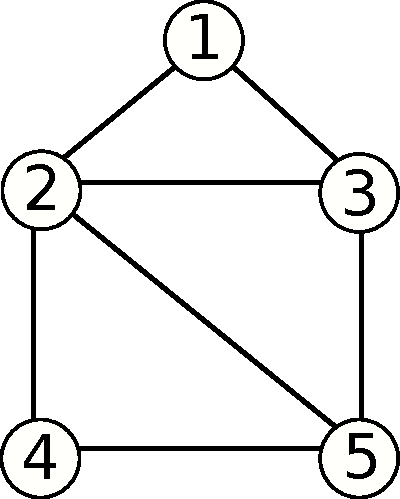
\includegraphics[height=40mm]{images/house.pdf}
\begin{exampleblock}{Beispiel}
	\begin{itemize}
		\item die Knotenfolge $1,2,3,5,2,3$ ist ein Weg aber kein Pfad, weil 2 und 3 zweimal vorkommen.
		\item die Folge $1,2,3,5,4$ ist ein Pfad
	\end{itemize}
	\end{exampleblock}
		\onslide<3>
		\begin{block}{Definition\hfill[Zusammenhangskomponenten]}
	\begin{itemize}
		\item f\"ur einen Graphen $G=(V,E)$ und $u,v\in V$ schreibe $u\sim_G v$, falls es einen Weg von $u$ nach $v$ gibt.
		\item die Relation $\sim_G$ ist eine \"Aquivalenzrelation, d.h.
			\begin{align*}
				u&\sim_G u&&\mbox{f\"ur alle }u\in V\\
				u&\sim_G v\ \Leftrightarrow\ v\sim_Gu&&\mbox{f\"ur alle }u,v\in V\\
u&\sim_G v\mbox{ und }v\sim_G w\ \Rightarrow\ u\sim_G w&&\mbox{f\"ur alle }u,v,w\in V
			\end{align*}
		\item die \"Aquivalenzklassen nennen wir \alert{Zusammenhangskomponenten} von $G$
		\item zwei Knoten liegen also genau dann in derselben Zusammenhangskomponente, wenn es einen Weg vom einen zum anderen gibt
	\end{itemize}
	\end{block}
		\onslide<4>
		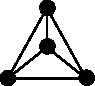
\includegraphics[height=20mm]{images/k4.pdf}\hfill
		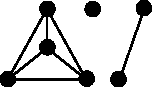
\includegraphics[height=20mm]{images/k4plusStuff.pdf}
\begin{exampleblock}{Zusammenhangskomponenten}
	\begin{itemize}
		\item ein Graph ist \alert{zusammenh\"angend}, wenn er nur eine Zusammenhangskomponente hat
		\item der linke Graph ist also zusammenh\"angend
		\item der rechte Graph ist unzusammenh\"angend
		\item der rechte Graph besteht aus drei Zusammenhangskomponenten
	\end{itemize}
	\end{exampleblock}
		\onslide<5>
		\hfill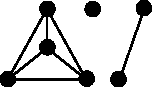
\includegraphics[height=20mm]{images/k4plusStuff.pdf}
\begin{exampleblock}{Zusammenhangskomponenten}
	\begin{itemize}
		\item ein \alert{isolierter Knoten} in einem Graphen ist eine Zusammenhangskomponente, die nur aus einem Knoten besteht
		\item eine \alert{isolierte Kante} ist eine Zusammenhangskomponente, die nur eine Kante enth\"alt
	\end{itemize}
	\end{exampleblock}
	\end{overprint}
\end{frame}

\begin{frame}\frametitle{\mytitle}
	\begin{overprint}
		\onslide<1>
		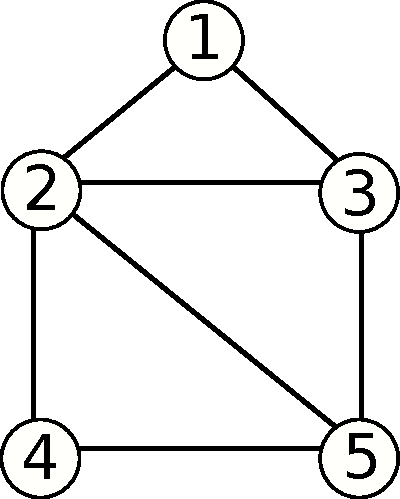
\includegraphics[height=30mm]{images/house.pdf}\hfill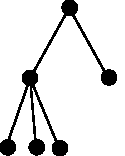
\includegraphics[height=30mm]{images/tree1.pdf}
		\begin{exampleblock}{Kreise in Graphen}
			\begin{itemize}
				\item ein \alert{Kreis} in einem Graphen $G$ ist eine Kopie eines Kreises $C_\ell$, $\ell\geq3$, die in $G$ enthalten ist
				\item der linke Graph enth\"alt also drei Kreise der L\"angen 3,4,5
				\item ein Graph ist \alert{kreisfrei}, wenn er keine Kreise enth\"alt
				\item der rechte Graph ist kreisfrei
			\end{itemize}
		\end{exampleblock}
		\onslide<2>
		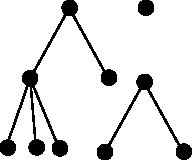
\includegraphics[height=30mm]{images/forest.pdf}\hfill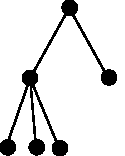
\includegraphics[height=30mm]{images/tree1.pdf}
		\begin{block}{Definition}
			\begin{itemize}
				\item ein kreisfreier Graph ist ein \alert{Wald}
				\item ein zusammenh\"anender Wald ist ein \alert{Baum}
			\end{itemize}
		\end{block}
		\onslide<3>
		\begin{exampleblock}{Bemerkungen}
			\begin{itemize}
				\item der kleinste Wald besteht nur aus einem Knoten	
				\item der Graph, der nur aus einer Kante besteht, ist ebenfalls ein Baum
				\item jeder Pfad ist ein Baum
				\item ein \alert{Blatt} in einem Wald ist ein Knoten vom Grad 1
			\end{itemize}
		\end{exampleblock}
	\end{overprint}
\end{frame}

\begin{frame}\frametitle{\mytitle}
		\hfill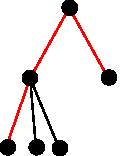
\includegraphics[height=30mm]{images/tree2.pdf}
	\begin{overprint}
		\onslide<1>
		\begin{block}{Lemma}
			Jeder Baum $G=(V,E)$ mit $E\neq\emptyset$ enth\"alt mindestens zwei Bl\"atter.
		\end{block}
		\onslide<2>
		\begin{exampleblock}{Beweis}
			\begin{itemize}
				\item betrachte einen l\"angsten Pfad $p=v_1,\ldots,v_\ell$.
				\item alle Nachbarn von $v_1$ und $v_\ell$ liegen auf $p$, weil man den Pfad sonst verl\"angern k\"onnte.
				\item wenn $v_1$ zwei Nachbarn h\"atte, w\"urden beide auf dem Pfad liegen; aber dann enthielte $G$ einen Kreis
			\end{itemize}
		\end{exampleblock}
		\onslide<3>
		\begin{exampleblock}{Beweis (fortgesetzt)}
			\begin{itemize}
				\item genauso f\"ur $v_\ell$
				\item also sind $v_1$ und $v_\ell$ Bl\"atter
			\end{itemize}
		\end{exampleblock}
	\end{overprint}
\end{frame}

\begin{frame}\frametitle{\mytitle}
	\begin{overprint}
		\onslide<1>
		\begin{block}{Proposition}
			Die folgenden Aussagen sind \"aquivalent.
			\begin{enumerate}
				\item der Graph $G=(V,E)$ ist ein Baum
				\item $G$ ist zusammenh\"angend und $|E|=|V|-1$
				\item $G$ ist kreisfrei und $|E|=|V|-1$
				\item $G$ ist kantenmaximal kreisfrei
				\item $G$ ist kantenminimal zusammenh\"angend
				\item in $G$ gibt es zu je zwei Knoten $v,w$ genau einen Pfad von $v$ nach $w$
			\end{enumerate}
		\end{block}
		\onslide<2>
		\begin{exampleblock}{Beweis \hfill[1 $\Rightarrow$ 2]}
			\begin{itemize}
				\item Induktion nach $n=|V|$
				\item f\"ur $n=1,2$ ist nichts zu zeigen
				\item f\"ur $n>2$ finde ein Blatt $v$ in $G$
				\item der Graph $G-\cbc v$ ist ein Baum
				\item nach Induktion gilt $$|E|-1=|E(G-\cbc v)|=|V(G-\cbc v)|-1=|V|-2$$
				\item folglich $|E|=|V|-1$
				\item per Definition ist $G$ zusammenh\"angend
			\end{itemize}
		\end{exampleblock}
		\onslide<3>
		\begin{exampleblock}{Beweis \hfill[2 $\Rightarrow$ 3]}
			\begin{itemize}
				\item Induktion nach $n=|V|$
				\item f\"ur $n=1,2$ ist nichts zu zeigen
				\item weil $$\sum_{v\in V}d_G(V)=2|E|=2(n-1),$$ gibt es einen Knoten $v\in V$ vom Grad~1
				\item der Graph $G'=G-\cbc v$ ist zusammenh\"angend und $|E(G')|=|V(G')|-1$
				\item also ist $G'$ nach Induktion kreisfrei
				\item folglich ist auch $G$ kreisfrei
				\item nach Annahme gilt $|V(G)|=|E(G)|-1$
			\end{itemize}
		\end{exampleblock}
		\onslide<4>
		\begin{exampleblock}{Beweis \hfill[3 $\Rightarrow$ 4]}
			\begin{itemize}
				\item Induktion nach $n=|V|$; f\"ur $n=1,2$ ist nichts zu zeigen
				%\item weil $$\sum_{v\in V}d_G(V)=2|E|=2(n-1),$$ gibt es einen Knoten $v\in V$ vom Grad~1
				\item weil $G$ kreisfrei ist, sind Anfangs- und Endknoten eines l\"angsten Pfades Bl\"atter
				\item $G$ enth\"alt also ein Blatt $v$
				\item der Graph $G'=G-\cbc v$ ist kreisfrei und $|E(G')|=|V(G')|-1$
				\item also ist $G'$ nach Induktion maximal kreisfrei
				\item somit ist $G'$ zusammenh\"angend; denn sonst k\"onnte man eine Kante zwischen zwei Komponenten von $G'$ hinzuf\"ugen
				\item daher kann man keine mit $v$ inzidente Kante hinzuf\"ugen, ohne einen Kreis zu schlie\ss en
			\end{itemize}
		\end{exampleblock}
		\onslide<5>
		\begin{exampleblock}{Beweis \hfill[4 $\Rightarrow$ 5]}
			\begin{itemize}
				\item weil $G$ kantenmaximal kreisfrei ist, ist $G$ zusammenh\"angend
				\item angenommen man k\"onnte eine Kante $e=vw$ l\"oschen, ohne den Zusammenhang zu zerst\"oren
				\item dann liegen $v,w$ in derselben Komponente von $G'=G-\cbc{e}$
				\item also schlie\ss t $e$ einen Kreis, Widerspruch
			\end{itemize}
		\end{exampleblock}
		\onslide<6>
		\begin{exampleblock}{Beweis \hfill[5 $\Rightarrow$ 6]}
			\begin{itemize}
				\item weil $G$ zusammenh\"angend ist, gibt es f\"ur alle $v,w\in V$ es einen Pfad von $v$ nach $w$
				\item angenommen zu $v,w$ gibt es zwei verschiedene Pfade $p\neq p'$
				\item dann gibt es eine Kante $e$ auf $p$, die nicht auf $p'$ vorkommt
				\item also ist $G-\cbc e$ zusammenh\"angend
				\item Widerspruch zur Annahme, $G$ sei kantenminimal zusammenh\"angend
			\end{itemize}
		\end{exampleblock}
		\onslide<7>
		\begin{exampleblock}{Beweis \hfill[6 $\Rightarrow$ 1]}
			\begin{itemize}
				\item Induktion nach $n=|V|$
				\item f\"ur $n=1,2$ ist nichts zu zeigen; sei also $n\geq3$
				\item betrachte einen l\"angsten Pfad $p=v_1\cdots v_\ell$ in $G$
				\item alle Nachbarn von $v_1$ und $v_\ell$ liegen auf $p$
				\item weil $p$ der einzige Pfad von $v_1$ nach $v_\ell$ ist, folgt, da\ss\ $v_1,v_\ell$ Bl\"atter sind
				\item weil in $G'=G-\cbc{v_1}$ je zwei Knoten durch genau einen Pfad verbunden sind, ist $G'$ ein Baum
				\item also ist auch $G$ ein Baum
			\end{itemize}
		\end{exampleblock}
	\end{overprint}
\end{frame}

\begin{frame}\frametitle{\mytitle}
	\begin{overprint}
		\onslide<1>
		\begin{block}{Definition}
			Ein \alert{spannender Baum} eines Graphen $G=(V,E)$ ist ein Untergraph $G'=(V,E')$ von $G$ mit derselben Knotenmenge wie $G$, der ein Baum ist.
		\end{block}
		\onslide<2>
		\begin{block}{Lemma}
			Jeder zusammenh\"angende Graph enth\"alt einen spannenden Baum.
		\end{block}
		\begin{exampleblock}{Beweis}
			\begin{itemize}
				\item Induktion nach der Kantenzahl von $G=(V,E)$
				\item wenn $G$ kantenminimal zusammenh\"angend ist, ist $G$ bereits selbst ein Baum
				\item sonst gibt es eine Kante $e\in E$, so da\ss\ $G'=G-\cbc e$ zusammenh\"angend ist
				\item nach Induktion besitzt $G'$ einen spannenden Baum
			\end{itemize}
		\end{exampleblock}
		\onslide<3>
		\begin{exampleblock}{Breiten- und Tiefensuche}
			\begin{itemize}
				\item wir lernen zwei Algorithmen kennen, die in einem zusammenh\"angenden Graphen spannende B\"aume bestimmen
				\item dar\"uber hinaus bestimmen diese Algorithmen die Zusammenhangskomponenten des Eingabegraphen
				\item die Eingabe ist jeweils ein Graph, der als Adjazenzliste gegeben ist
			\end{itemize}
		\end{exampleblock}
		\onslide<4>
		\begin{exampleblock}{Breiten- und Tiefensuche}
			\begin{itemize}
				\item in einem Graphen $G$ definieren wir den \alert{Abstand} von $v,w\in V(G)$ als
					\begin{align*}
						\dist_G(v,w)=\min_{\ell\geq0}\exists\mbox{ Weg der L\"ange $\ell$ von $v$ nach $w$}
					\end{align*}
				\item falls $v,w$ in verschiedenen Zusammenhangskomponenten liegen, verwenden wir die Konvention
					$$\dist_G(v,w)=\infty$$
			\end{itemize}
		\end{exampleblock}
	\end{overprint}
\end{frame}

\begin{frame}\frametitle{\mytitle}
	\begin{overprint}
		\onslide<1>
		\begin{exampleblock}{{\tt BFS}$(G,s)$}
			\begin{enumerate}
				\item F\"arbe alle Knoten $v\in V(G)\setminus\cbc s$ gr\"un und f\"arbe $s$ gelb.
				\item Setze $d(v)=\infty$ f\"ur alle $v\in V(G)\setminus\cbc s$ und setze $d(s)=0$.
				\item Setze $p(v)=\emptyset$ f\"ur alle $v\in V$.
				\item Lege eine Warteschlange $Q$ an und f\"uge $s$ in $Q$ ein.
				\item Solange $Q$ nicht leer ist,
				\item $\quad$entnehme $v$ aus $Q$
				\item $\quad$f\"arbe $v$ rot
				\item $\quad$f\"ur alle $u\in\partial v$ mit Farbe gr\"un
				\item $\quad\quad$f\"arbe $u$ gelb, setze $p(u)=v$, $d(u)=d(v)+1$ und f\"uge $u$ in $Q$ ein
			\end{enumerate}		
		\end{exampleblock}
		\onslide<2>
		\begin{block}{Satz}
			{\tt BFS} hat Laufzeit $O(|V(G)|+|E(G)|)$.
			Bei Beendigung des Algorithmus' gilt folgendes.
			\begin{enumerate}[(i)]
				\item Die Zusammehangskomponente des Startknotens $s$ besteht aus genau den Knoten $v$, f\"ur die $d(v)<\infty$.
				\item F\"ur alle $v\in V(G)$ gilt $d(v)=\dist_G(s,v)$.
				\item Der Untergraph $$(\{v\in V(G):d(v)<\infty\},\{\{v,p(v)\}:v\in V(G),\,p(v)\neq\emptyset\})$$ ist ein spannender Baum der Zusammehangskomponente von $s$ in $G$.
			\end{enumerate}
		\end{block}
		\onslide<3>
		\begin{block}{Handschlaglemma}
			F\"ur jeden Graphen $G$ gilt
			\begin{align*}
				\sum_{v\in V(G)}d_v(G)=2|E(G)|.
			\end{align*}
		\end{block}
		\onslide<4>
		\begin{block}{Lemma~1}
			{\tt BFS} hat Laufzeit $O(|V(G)|+|E(G)|)$.
		\end{block}
		\begin{exampleblock}{Berweis}
			\begin{itemize}
				\item Laufzeit der Schritte (1)--(4) betr\"agt $O(|V(G|)$.
				\item Jeder Knoten wechselt h\"ochstens zweimal seine Farbe, und zwar von gr\"un auf gelb auf rot.
				\item Deshalb wird kein Knoten mehrmals in $Q$ eingef\"ugt, und folglich auch nicht wieder entnommen.
				\item Aus diesem Grund ist die Laufzeit der Hauptschleife (5)--(9) beschr\"ankt durch $O(|V(G)|)+\sum_{v\in V(G)}d_G(v)=O(|V(G)|)+O(|E(G)|)$
			\end{itemize}
		\end{exampleblock}
		\onslide<5>
		\begin{block}{Lemma~2}
			W\"ahrend der gesamten Ausf\"uhrung von {\tt BFS} gilt 
			\begin{align*}
				d(v)\geq\dist_G(s,v)\qquad\mbox{f\"ur alle Knoten $v$}.
			\end{align*}
		\end{block}
		\onslide<6>
		\begin{exampleblock}{Beweis}
			\begin{itemize}
				\item Wir f\"uhren Induktion nach der Zahl der Iterationen der Hauptschleife (5)--(9).
				\item Anfangs gilt $d(v)=\infty$ f\"ur alle $v\in V(G)\setminus\cbc s$, weshalb die Behauptung trivial erf\"ullt ist.
				\item Betrachte nun den n\"achsten Knoten $v$, der aus $Q$ entnommen wird, sowie einen gr\"unen Nachbarn $u$ von $v$
				\item	Dann gilt $d(u)=d(v)+1$.
				\item Andererseits gilt offensichtlich $\dist_G(s,u)\leq\dist_G(s,v)+1$, weil ein Pfad von $s$ nach $v$ um eine Kante nach $u$ verl\"angert werden kann.
				\item Weil $d(v)\geq\dist_G(s,v)$ nach Induktionsvoraussetzung, schlie\ss en wir, da\ss\ $d(u)\geq\dist_G(s,u)$ f\"ur alle gr\"unen $u\in\partial_Gv$.
			\end{itemize}
		\end{exampleblock}
		\onslide<7>
		\begin{block}{Lemma~3}
			Angenommen die Warteschlange $Q$ enth\"alt die Knoten $q_1,\ldots,q_\ell$.
			Dann gilt 
			\begin{align*}
				d(q_1)\leq\cdots\leq d(q_\ell)\leq d(q_1)+1.
			\end{align*}
			Wird ferner ein Knoten $u$ vor einem anderen Knoten $u'$ in $Q$ eingef\"ugt, so gilt $$d(u)\leq d(u').$$
		\end{block}
		\onslide<8>
		\begin{exampleblock}{Beweis}
			\begin{itemize}
				\item Wir f\"uhren Induktion nach der Zahl der Iterationen der Hauptschleife.
				\item Zu Beginn enth\"alt $Q$ nur den Knoten $s$, so da\ss\ nichts zu zeigen ist.
				\item Es ist klar, da\ss\ die Ungleichung nach einer Ausf\"uhrung von Schritt (6) erhalten bleibt.
				\item Betrachte ferner eine Ausf\"uhrung von Schritt (9).
				\item Dann gilt nach Induktionsvoraussetzung f\"ur den neu eingef\"ugten Knoten $v$, da\ss\ $d(v)=d(v_1)+1\geq d(v_2)$.
				\item Also bleibt die Ungleichung erhalten.
				\item Die zweite Behauptung folgt unmittelbar aus der Ungleichung.
			\end{itemize}
		\end{exampleblock}
		\onslide<9>
		\begin{exampleblock}{Beweis}
			\begin{itemize}
				\item Die behauptete Laufzeit ergibt sich unmittelbar aus Lemma~1
				\item Wir zeigen (ii), woraus (i) direkt folgt
				\item Nach Lemma~2 gen\"ugt zu zeigen, da\ss\ $d(u)\leq\dist_G(s,u)$ f\"ur alle $u$ bei Beendigung von {\tt BFS}
				\item \emph{Beweis durch Widerspruch:} nimm an, es g\"abe ein $u$ mit
					$$d(u)>\dist_G(s,u)$$
			\end{itemize}
		\end{exampleblock}
		\onslide<10>
		\begin{exampleblock}{Beweis}
			\begin{itemize}
				\item W\"ahle $u\neq s$ so, da\ss\ $\dist_G(s,u)$ kleinstm\"oglich
				\item Da $d(u)>\dist_G(s,u)$ gilt $\dist_G(s,u)<\infty$
				\item Also gibt es einen k\"urzesten Pfad $P$ von $s$ nach $u$
				\item Sei $v$ der letzte vor $u$ auf $P$; dann $\dist_G(u)=\dist_G(v)+1$
				\item Da $\dist_G(s,v)<\dist_G(s,u)$, folgt $d(v)=\dist_G(v)$
				\item In Schritten (8)--(12) bei Entnahme von $v$ mu\ss\ $u$ gelb oder rot gef\"arbt sein
				\item Daher zeigt Lemma~3, da\ss\ $d(u)\leq d(v)+1\leq\dist_G(u)$
				\item Dies ist ein Widerspruch, also ist (ii) bewiesen
				\item Aussage (iii) ergibt sich direkt aus (i) und (ii)
			\end{itemize}
		\end{exampleblock}
	\end{overprint}
\end{frame}

\begin{frame}\frametitle{\mytitle}
	\begin{overprint}
		\onslide<1>
		\begin{exampleblock}{{\tt DFS}$(G)$}
			\begin{enumerate}
				\item F\"arbe alle Knoten $v\in V(G)$ gr\"un.
				\item Setze $c(v)=0$ und $p(v)=\emptyset$ f\"ur alle $v\in V$.
				\item Setze $j=1$
				\item F\"ur alle $v\in V(G)$
				\item $\quad$falls $v$ gr\"un gef\"arbt ist
				\item $\quad\quad$f\"uhre {\tt DFSLoop}$(G,v,j)$ aus.
				\item $\quad\quad$Erh\"ohe $j$ um $1$.
			\end{enumerate}
		\end{exampleblock}
		\onslide<2>
		\begin{exampleblock}{{\tt DFSLoop}$(G,v,j)$}
			\begin{enumerate}
				\item F\"arbe $v$ gelb und setze $c(v)=j$.
				\item F\"ur alle $u\in\partial_Gv$
				\item $\quad$Falls $u$ gr\"un ist
				\item $\quad\quad$Setze $p(u)=v$.
				\item $\quad\quad$F\"uhre {\tt DFSLoop}$(G,u,j)$ aus.
				\item F\"arbe $v$ rot.
			\end{enumerate}
		\end{exampleblock}
		\onslide<3>
		\begin{block}{Satz}
			\begin{itemize}
				\item {\tt DFS} hat Laufzeit $O(|V(G)|+|E(G)|)$.
				\item Die Mengen $c^{-1}(j)$ f\"ur $j\geq1$ bilden genau die Zusammehangskomponenten von $G$.
			\end{itemize}
		\end{block}
	\end{overprint}
\end{frame}

\begin{frame}\frametitle{\mytitle}
	\begin{exampleblock}{Zusammenfassung}
		\begin{itemize}
			\item der Zusammenhangsbegriff
			\item B\"aume und W\"alder
			\item Breitensuche
			\item Tiefensuche
		\end{itemize}
	\end{exampleblock}
\end{frame}

\end{document}
